\section{Geschichteter Kondensator}

Ein geschichteter Plattenkondensator lässt sich mit verschiedenen Programmen graphisch darstellen und analysieren. Während FEMM auf eine zwei Dimensionale Darstellung des Problems beschränkt ist, lassen sich mit Hilfe der Methode der Finiten Integration (FIT) und einem geeigneten Simulationsprogramm drei Dimensionale Darstellungen erzeugen. Das angehängte Skript \tt{SkriptAg8\_2} bildet den Vorgang der FIT ab, die Ergebnisse werden in ParaView graphisch dargestellt.\\ \\
Zur Berechnung wird das Gebiet $\Omega = \{-1,1\}^3$ betrachtet, es gilt $N_x = N_y = N_z = 21$ und damit $Np = 9261$, dieses Gebiet wird kanonisch nummeriert. Allgemein wird ein Plattenkondensator mit linear-variierender Permittivität nachgestellt, die unterschiedlichen Permittivitäten werden mit der Methode \tt{calc\_eps\_linear} bestimmt und in einem Vektor gespeichert. Des Weiteren ist an den Knoten, die die Elektroden widerspiegeln eine \textsc{Dirichlet}-Randbedingung vorgegeben. Das Potential an diesen Knoten beträgt jeweils \SI{0}{\volt} bzw. \SI{1}{\volt}. Das elektrische Feld und die Potentiale zwischen den beiden Elektroden gilt es zu berechnen. \\ \\
Die Methode \tt{createMeps} liefert die zur Rechnung benötigte Matrix $\mb{M}_\epsilon$, sie führt eine Materialmittlung durch. Um nun alle Potentiale in dem Gebiet $\Omega$ zu berechnen, muss das Gleichungssystem 
\begin{equation}
	\tilde{\mb{S}}\mb{M}_\epsilon\tilde{\mb{S}}^T\mb{\Phi} = 0
	\label{eq:meps}
\end{equation} berechnet werden. Zur Vereinfachung nimmt man an, dass $\mb{A} = \tilde{\mb{S}}\mb{M}_\epsilon\tilde{\mb{S}}^T$ gilt. Durch diese Rechnung wird garantiert, dass nur im Rechengebiet befindliche Gitterkanten und keine Geisterkanten beachtet werden, die Struktur der Matrix ist in Abbildung \ref{fig:MatA} zu sehen.\\ \\
In $\mb{\Phi}$ befinden sich sowohl die bekannten Potentiale der Randbedingungen, als auch die noch unbekannten Potentiale. Ist das Potential $\phi_n$ an einem Knoten $P_n$ des Gitters bekannt, so kann die $n$-te Zeile und Spalte der Matrix \b{A} gestrichen werden, sowie der $n$-te Eintrag aus dem Vektor $\mb{\Phi}$.\\
Die $n$-te Spalte, abzüglich des Eintrags in der $n$-ten Zeile, der Matrix \b{A} wird auf der anderen Seite des Gleichungssystems (\ref{eq:meps}) abgezogen und mit dem bekannten $\phi_n$ multipliziert. Führt man dies nun für alle Punkte durch, bei denen die Randbedingung bekannt ist, so entsteht ein Gleichungssystem der Form 
\begin{equation*}
	\mb{A}_{11}\mb{x}_1 = -\mb{A}_{12}\mb{x}_2,
\end{equation*} 
wobei in $\mb{x}_1$ alle nicht bekannten und in $\mb{x}_2$ alle bekannten Potentiale gespeichert sind. $\mb{x}_1$ lässt sich nun in Matlab ganz einfach mit $$\mb{x}_1 = -\mb{A}_{11}\backslash\mb{A}_{12}\mb{x}_2$$ berechnen. Der Potentialvektor $\mb{\Phi}$ kann aus $\mb{x}_1$ und $\mb{x}_2$ in der richtigen Reihenfolge bestimmt werden. Das dazugehörige elektrische Feld wird mit $\tilde{\mb{S}}^T\mb{\Phi} = \mb{\overset{\frown}{e}}$ berechnet. Da es sich bei $\mb{\overset{\frown}{e}}$ um eine Potentialdifferenz mit der Einheit Volt handelt, teilt man noch durch den räumlichen Abstand der beiden Gitterpunkte, um auf ein angenähertes elektrische Feld zu bestimmen.
\newpage
\begin{figure}[h]
	\vspace*{-38pt}
	\begin{subfigure}{.49\textwidth}
		\centering
		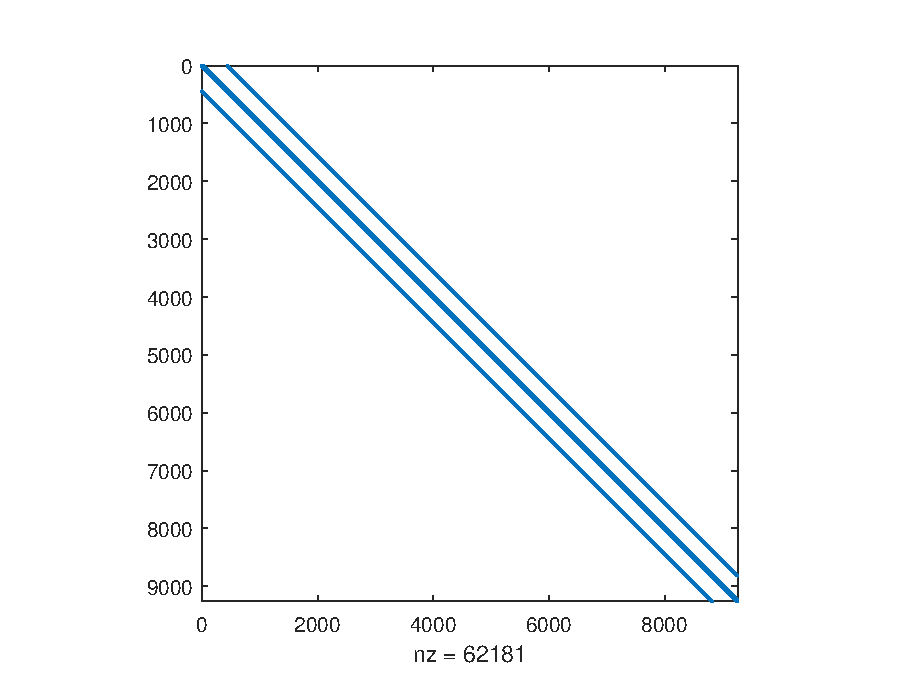
\includegraphics[width=\textwidth]{data/Ag8_2MatrixA}
		\caption{Die Systemmatrix, die bei $N_x = N_y = N_z = 21$ entsteht}
		\label{fig:MatA}
	\end{subfigure}
	\begin{subfigure}{.49\textwidth}
		\centering
		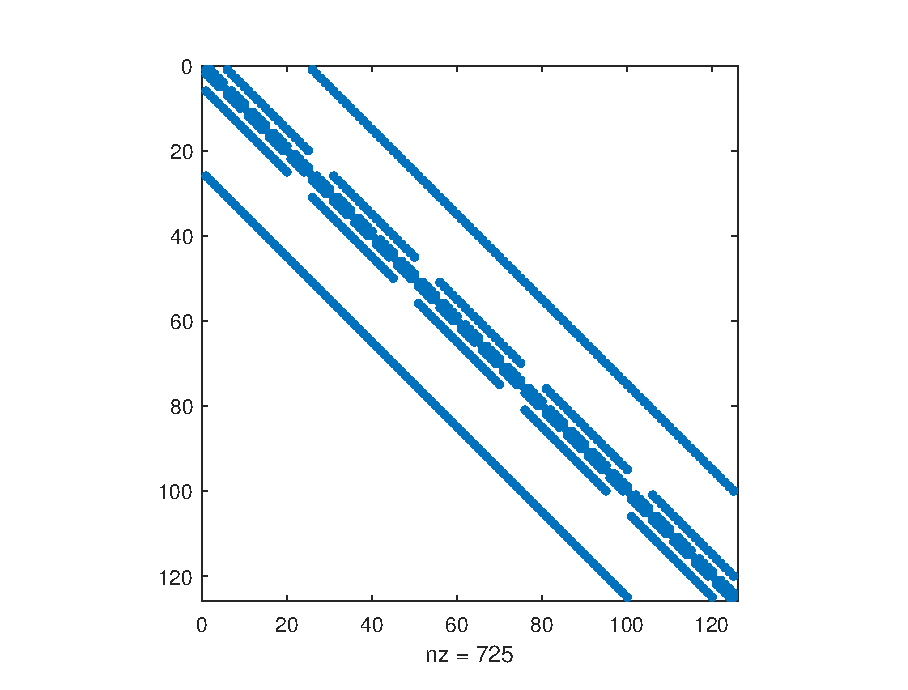
\includegraphics[width=\textwidth]{data/Ag8_2MatrixAkleiner}
		\caption{Die Systemmatrix, die bei $N_x = N_y = N_z = 5$ entsteht}
	\end{subfigure}
\end{figure}
In Abbildung \ref{fig:Eps2} und \ref{fig:Eps10} sind verschiedene Potentialverläufe zu sehen, bei Abb. \ref{fig:Eps2} wurde eine linear ansteigende Permittivität $\varepsilon_r \in [1,2]$ gewählt, Abb. \ref{fig:Eps10} wiederum beschreibt das Potential mit $\varepsilon_r \in [1,10]$.\\
Abbildung \ref{fig:EFeld} zeigt das vorher berechnete elektrische Feld. Dieses hat nicht den erwarteten Verlauf, bei der Rechnung $\tilde{\mb{S}}^T\mb{\Phi} = \mb{\overset{\frown}{e}}$ werden Geisterkanten beachtet, die das Ergebnis verfälschen, zudem müssen die Werte auf eine Zelle gemittelt werden. Zunächst wird eine Indexmenge bestimmt, die die Indizes aller primären Volumina, die vollständig im Rechengebiet liegen beinhaltet. In dem Skript \tt{SkriptAg8\_2} geschieht dieser Vorgang in drei in sich geschachtelten Vorschleifen (Zeile 32 bis 45). Grafisch interpretiert, geht man zunächst alle Volumen in $x$-Richtung bis zum Index $N_x-1$ durch und speichert diese Indizes. Hat man $N_x-1$ erreicht geht man einen Schritt in $y$-Richtung und wiederholt die Zählung in $x$-Richtung. Diesen Vorgang wird $N_y-1$ mal wiederholt, bis man die nächste Stufe in $z$-Richtung erreicht.  Auch in $z$-Richtung wird die Zählung $N_z-1$ mal durchgeführt.
\begin{figure}[h!]
	\vspace*{-10pt}
	\begin{subfigure}{.45\textwidth}
		\centering
		\includegraphics[width=\textwidth]{data/Ag8_2eps2}
		\caption{Potentialverteilung im Kondensator mit $\varepsilon_r \in [1,2]$}
		\label{fig:Eps2}
	\end{subfigure}
	\begin{subfigure}{.45\textwidth}
		\centering
		\includegraphics[width=\textwidth]{data/Ag8_2eps10}
		\caption{Potentialverteilung im Kondensator mit $\varepsilon_r \in [1,10]$}
		\label{fig:Eps10}
	\end{subfigure}
	\centering
	\begin{subfigure}{.45\textwidth}
		\centering
		\includegraphics[width=\textwidth]{data/Ag8_2Efeld}
		\caption{Mit dem dualen Divergenzoperator $\tilde{\mb{S}}^T\mb{\Phi}$ berechnete elektrische Feld}
		\label{fig:EFeld}
	\end{subfigure}
\end{figure}
\newpage
Nun können der Methode \tt{fit\_pe2pc} die passenden Indizes übergeben werden und das elektrische Feld somit berechnet werden. Das daraus resultierende Ergebnis ist in Abbildung \ref{fig:EFeldM} dargestellt.
\begin{figure}[h]
	\centering
	\includegraphics[width=\textwidth]{data/Ag8_2EfeldMittel}
	\caption{Mit dem dualen Divergenzoperator $\tilde{\mb{S}}^T$ und dem Potential $\mb{\Phi}$ berechnete elektrische Feld mit anschließender Mittelung auf die Zellen}
	\label{fig:EFeldM}
\end{figure}